%package list
\documentclass{article}
\usepackage[top=3cm, bottom=3cm, outer=3cm, inner=3cm]{geometry}
\usepackage{multicol}
\usepackage{graphicx}
\usepackage{url}
%\usepackage{cite}
\usepackage{hyperref}
\usepackage{array}
%\usepackage{multicol}
\newcolumntype{x}[1]{>{\centering\arraybackslash\hspace{0pt}}p{#1}}
\usepackage{natbib}
\usepackage{pdfpages}
\usepackage{multirow}
\usepackage[normalem]{ulem}
\useunder{\uline}{\ul}{}
\usepackage{svg}
\usepackage{xcolor}
\usepackage{listings}
\lstdefinestyle{ascii-tree}{
	literate={├}{|}1 {─}{--}1 {└}{+}1 
}
\lstset{basicstyle=\ttfamily,
	showstringspaces=false,
	commentstyle=\color{red},
	keywordstyle=\color{blue}
}
%\usepackage{booktabs}
\usepackage{caption}
\usepackage{subcaption}
\usepackage{float}
\usepackage{array}

\newcolumntype{M}[1]{>{\centering\arraybackslash}m{#1}}
\newcolumntype{N}{@{}m{0pt}@{}}


%%%%%%%%%%%%%%%%%%%%%%%%%%%%%%%%%%%%%%%%%%%%%%%%%%%%%%%%%%%%%%%%%%%%%%%%%%%%
%%%%%%%%%%%%%%%%%%%%%%%%%%%%%%%%%%%%%%%%%%%%%%%%%%%%%%%%%%%%%%%%%%%%%%%%%%%%
\newcommand{\itemEmail}{jchuraaca@unsa.edu.pe}
\newcommand{\itemStudent}{Julio Rubén Chura Acabana}
\newcommand{\itemCourse}{ F. de Programción 2}
\newcommand{\itemCourseCode}{20230472}
\newcommand{\itemSemester}{I}
\newcommand{\itemUniversity}{Universidad Nacional de San Agustín de Arequipa}
\newcommand{\itemFaculty}{Facultad de Ingeniería de Producción y Servicios}
\newcommand{\itemDepartment}{Departamento Académico de Ingeniería de Sistemas e Informática}
\newcommand{\itemSchool}{Escuela Profesional de Ingeniería de Sistemas}
\newcommand{\itemAcademic}{2023 - B}
\newcommand{\itemInput}{Del 6 Noviembre 2023}
\newcommand{\itemOutput}{Al 13 Noviembre 2023}
\newcommand{\itemPracticeNumber}{09}
\newcommand{\itemTheme}{Definición de Clases de Usuario
	Clase Soldado}
%%%%%%%%%%%%%%%%%%%%%%%%%%%%%%%%%%%%%%%%%%%%%%%%%%%%%%%%%%%%%%%%%%%%%%%%%%%%
%%%%%%%%%%%%%%%%%%%%%%%%%%%%%%%%%%%%%%%%%%%%%%%%%%%%%%%%%%%%%%%%%%%%%%%%%%%%

\usepackage[english,spanish]{babel}
\usepackage[utf8]{inputenc}
\AtBeginDocument{\selectlanguage{spanish}}
\renewcommand{\figurename}{Figura}
\renewcommand{\refname}{Referencias}
\renewcommand{\tablename}{Tabla} %esto no funciona cuando se usa babel
\AtBeginDocument{%
	\renewcommand\tablename{Tabla}
}

\usepackage{fancyhdr}
\pagestyle{fancy}
\fancyhf{}
\setlength{\headheight}{30pt}
\renewcommand{\headrulewidth}{1pt}
\renewcommand{\footrulewidth}{1pt}
\fancyhead[L]{\raisebox{-0.2\height}{
\includegraphics[width=3cm]{img/logo_episunsa.png}}}
\fancyhead[C]{\fontsize{7}{7}\selectfont	\itemUniversity \\ \itemFaculty \\ \itemDepartment \\ \itemSchool \\ \textbf{\itemCourse}}
\fancyhead[R]{\raisebox{-0.2\height}{
\includegraphics[width=1.2cm]{img/logo_abet}}}
\fancyfoot[L]{Estudiante Julio Rubén Chura Acabana}
\fancyfoot[C]{\itemCourse}
\fancyfoot[R]{Página \thepage}

% para el codigo fuente
\usepackage{listings}
\usepackage{color, colortbl}
\definecolor{dkgreen}{rgb}{0,0.6,0}
\definecolor{gray}{rgb}{0.5,0.5,0.5}
\definecolor{mauve}{rgb}{0.58,0,0.82}
\definecolor{codebackground}{rgb}{0.95, 0.95, 0.92}
\definecolor{tablebackground}{rgb}{0.8, 0, 0}

\lstset{frame=tb,
	language=bash,
	aboveskip=3mm,
	belowskip=3mm,
	showstringspaces=false,
	columns=flexible,
	basicstyle={\small\ttfamily},
	numbers=none,
	numberstyle=\tiny\color{gray},
	keywordstyle=\color{blue},
	commentstyle=\color{dkgreen},
	stringstyle=\color{mauve},
	breaklines=true,
	breakatwhitespace=true,
	tabsize=3,
	backgroundcolor= \color{codebackground},
}

\begin{document}
	
	\vspace*{10px}
	
	\begin{center}	
		\fontsize{17}{17} \textbf{ Informe de Laboratorio \itemPracticeNumber}
	\end{center}
	\centerline{\textbf{\Large Tema: \itemTheme}}
	%\vspace*{0.5cm}	
	
	\begin{flushright}
		\begin{tabular}{|M{2.5cm}|N|}
			\hline 
			\rowcolor{tablebackground}
			\color{white} \textbf{Nota}  \\
			\hline 
			\\[30pt]
			\hline 			
		\end{tabular}
	\end{flushright}	
	
	\begin{table}[H]
		\begin{tabular}{|x{4.7cm}|x{4.8cm}|x{4.8cm}|}
			\hline 
			\rowcolor{tablebackground}
			\color{white} \textbf{Estudiante} & \color{white}\textbf{Escuela}  & \color{white}\textbf{Asignatura}   \\
			\hline 
			{\itemStudent \par \itemEmail} & \itemSchool & {\itemCourse \par Semestre: \itemSemester \par Código: \itemCourseCode}     \\
			\hline 			
		\end{tabular}
	\end{table}		
	
	\begin{table}[H]
		\begin{tabular}{|x{4.7cm}|x{4.8cm}|x{4.8cm}|}
			\hline 
			\rowcolor{tablebackground}
			\color{white}\textbf{Laboratorio} & \color{white}\textbf{Tema}  & \color{white}\textbf{Duración}   \\
			\hline 
			\itemPracticeNumber & \itemTheme & 04 horas   \\
			\hline 
		\end{tabular}
	\end{table}
	
	\begin{table}[H]
		\begin{tabular}{|x{4.7cm}|x{4.8cm}|x{4.8cm}|}
			\hline 
			\rowcolor{tablebackground}
			\color{white}\textbf{Semestre académico} & \color{white}\textbf{Fecha de inicio}  & \color{white}\textbf{Fecha de entrega}   \\
			\hline 
			\itemAcademic & \itemInput &  \itemOutput  \\
			\hline 
		\end{tabular}
	\end{table}
	
	\section{Tarea}
	\begin{itemize}
		\item	 Crear 3 constructores sobrecargados.
		\item La actitud puede ser defensiva, ofensiva, fuga. Dicha actitud varía cuando el 
		soldado defiende, ataca o huye respectivamente.
		\item	Al atacar el soldado avanza, al avanzar aumenta su velocidad en 1. Al defender 
		el soldado se para. Al huir aumenta su velocidad en 2. Al retroceder, si su 
		velocidad es mayor que 0, entonces primero para y su actitud es defensiva, y 
		si su velocidad es 0 entonces disminuirá a valores negativos. Al ser atacado su 
		vida actual disminuye y puede llegar incluso a morir.
		\item Crear los atributos y métodos extra que considere necesarios.
		\item Tendrá 2 Ejércitos. Usar la estructura de datos que considere más adecuada. 
		Inicializar el tablero con n soldados aleatorios entre 1 y 10 para cada Ejército. 
		Cada soldado tendrá un nombre autogenerado: Soldado0X1, Soldado1X1, etc.,
		un valor de puntos de vida autogenerado aleatoriamente [1..5], la fila y 
		columna también autogenerados aleatoriamente (no puede haber 2 soldados 
		en el mismo cuadrado). Nivel de ataque y de defensa son aleatorios [1..5]. Se 
		debe mostrar el tablero con todos los soldados creados (usar caracteres) y distinguir los de un ejército de los del otro ejército. Además de 
		los datos del Soldado con mayor vida de cada ejército, el promedio de puntos 
		de vida de todos los soldados creados por ejército, los datos de todos los 
		soldados por ejército en el orden que fueron creados y un ranking de poder de 
		todos los soldados creados por ejército (del que tiene más nivel de vida al que 
		tiene menos) usando 2 diferentes algoritmos de ordenamiento. Finalmente, que 
		muestre qué ejército ganará la batalla (indicar la métrica usada para decidir al 
		ganador de la batalla). Hacerlo un programa iterativo.
		\item  Crear el diagrama de clases UML completo
	
		\item Usted debe realizar varios commits y al término de la actividad deberá realizar un informe.
		
		
	\end{itemize}
	
	\section{Equipos, materiales y temas utilizados}
	\begin{itemize}
		\item Sistema Operativo Windows
		\item Vim 9.0
		\item OpenJDK 64-Bits 20.0.2
		\item Git 2.42.0
		\item Cuenta en GitHub con el correo institucional
		\item Definición de Clases de Usuario Clase Soldado
	\end{itemize}
	
	\section{URL de Repositorio Github}
	\begin{itemize}
		\item URL del Repositorio GitHub para clonar o recuperar.
		\item \url{https://github.com/JulioChura/fp2-23b.git}
		\item URL para el laboratorio 01 en el Repositorio GitHub.
		\item \url{https://github.com/JulioChura/fp2-23b/tree/main/fase02/lab09}
	\end{itemize}
	
	\section{Actividades con el repositorio GitHub}
	


	\subsection{Inicialización del espacio de trabajo}
	
	\begin{lstlisting}[language=bash,caption={Inicializando el espacio de trabajo}][H]
		mkdir lab09
		cd ..
		cd lab07
		Copy-Item "Soldier.java" -Destination "..\lab09"
		Copy-Item "VideoJuego4.java" -Destination "..\lab09\VideoJueg06.java"
		cd ..
		cd lab09
		vim VideoJuego6.java	
	\end{lstlisting}
	
	\begin{lstlisting}[language=bash,caption={Commit: 24b299f6d4b3ebd17971adadc7057ab72724b41c }][H]
		git add VideoJuego6.java
		git commit -m "Se copia VideoJuego4.java del lab07 al lab09"
		git push -u origin main
	\end{lstlisting}
	
	\begin{lstlisting}[language=bash,caption={Commit: de2a4e5f1787deaab8683e2f4ca01a0d3922cd9e }][H]
		git add VideoJuego4.java
		git commit -m "Se copia Soldier.java del lab07 al lab09"
		git push -u origin main
	\end{lstlisting}
	
aaaaaaaaaaaaaaa
	
	\subsection{Funciones ya trabajadas en laboratorios pasados}

	\begin{figure}[H]
		\centering
		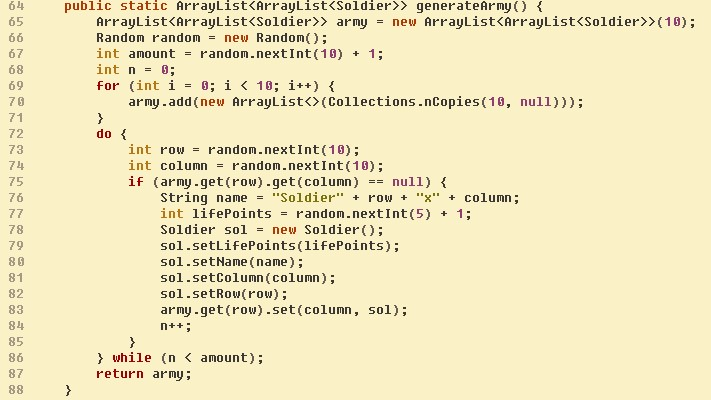
\includegraphics[width=1\textwidth,keepaspectratio]{img/generateArmy.jpg}
		%\includesvg{img/automata.svg}
		%\label{img:mot2}
		%\caption{Product backlog.}
	\end{figure}
	
	\begin{itemize}	
		
		\item Método generateArmy(): Crea un arreglo bidimensional de 10 filas y 10 columnas con
		el fin de cubrir la misma cantidad de casillas del tablero, por
		lo que habrán posiciones que quedarán vacías ya que la cantidad de elementos del arreglo será un número aleatoria que oscila entre 1 a 10. También se genera el nombre de cada Soldier y
		sus puntos de vida de forma aleatoria. Este arreglo nos servirá más que nada para imprimir el
		tablero de una forma más sencilla.
		\item Como sabemos, el ArrayList es una estructura de datos compacta, es decir puede recibir n cantidad de elementos y esos elementos se acomodarán, por lo que no hay posiciones con elementos vacíos, pero es posible inicializar algunas posiciones con ningún elemento, en nuestro caso null, y eso hace el primer for, se encarga de llenar el ArrayList con null.
	\end{itemize}
	
	
	\begin{figure}[H]
		\centering
		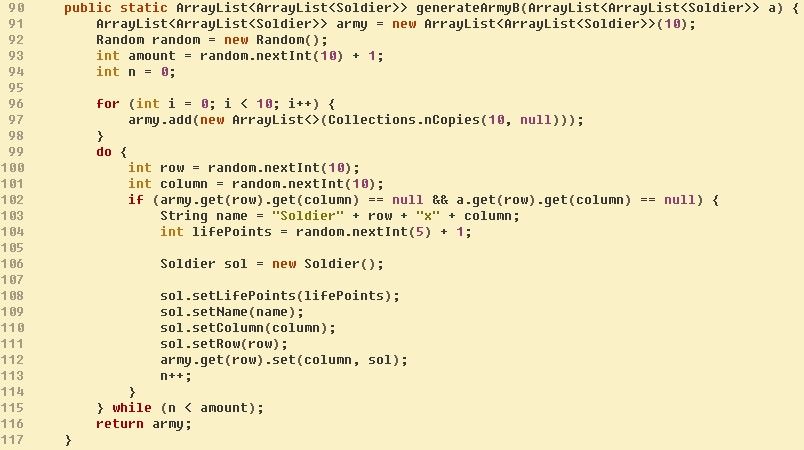
\includegraphics[width=1.1\textwidth,keepaspectratio]{img/generateArmyB.jpg}
		%\includesvg{img/automata.svg}
		%\label{img:mot2}
		%\caption{Product backlog.}
	\end{figure}
	
	\begin{itemize}	
		\item Método generateArmyB:La razón de la creación de este método se debe a que hay casos en los que la cantidad de fichas del ejército B que están ubicadas en el tablero no coincide en cantidad con lo que se genera. Básicamente este método es igual que generateArmy, solo que este recibe un parámetro de tipo ArrayList bidimensional- Soldier que se usará para verificar que se generen los soldados del ejército B sin que haya cruces con los del ejército A. Lo único que se añade al método generateArmy es a.get(row).get(column) == null
	\end{itemize}
	

	
	\begin{figure}[H]
		\centering
		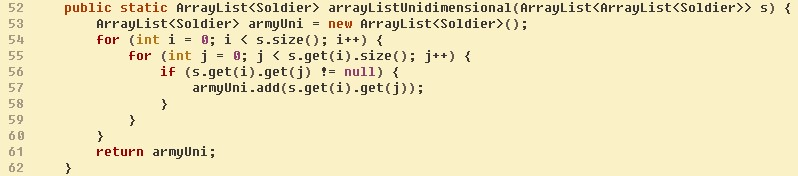
\includegraphics[width=1.1\textwidth,keepaspectratio]{img/arrayListUni.jpg}
		%\includesvg{img/automata.svg}
		%\label{img:mot2}
		%\caption{Product backlog.}
	\end{figure}
	
	\begin{itemize}	
		\item arrayListUnidimensional: A pesar de ya contar con dos ArrayList bidimensionales, se opta por transformarlos en ArrayList unidimensionales ya que nos facilitará trabajar con los demás métodos que la práctica de laboratorio solicita. En el main se hace la creación de dos ArrayList unidimensionales tanto para el ejército A y B.
	\end{itemize}
	
	\begin{figure}[H]
		\centering
		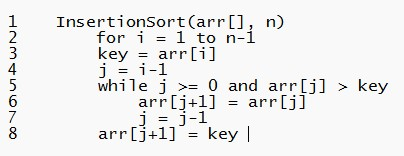
\includegraphics[width=0.8\textwidth,keepaspectratio]{img/insertion.jpg}
		%\includesvg{img/automata.svg}
		%\label{img:mot2}
		%\caption{Product backlog.}
	\end{figure}
	
	\begin{figure}[H]
		\centering
		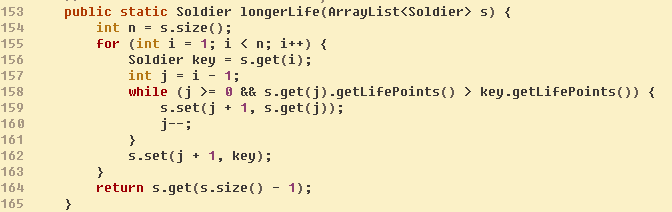
\includegraphics[width=1\textwidth,keepaspectratio]{img/longerLife.png}
		%\includesvg{img/automata.svg}
		%\label{img:mot2}
		%\caption{Product backlog.}
	\end{figure}
	
	
	\begin{itemize}	
		\item longerLife(): Se adapta el pseudocódigo de insertion y se le da la forma para que se aplique en un ArrayList. Lo que hace el método es ordenar de menor a mayor, por lo que último elemento es el mayor. El método devuelve al Soldier que se encuentra en esa posición.
		\item Se muestra el pseudocódigo, pero aplicado a un arreglo Estándar. A pesar de ser otra estructura, la idea es la misma
	\end{itemize}
		
		
	\begin{figure}[H]
		\centering
		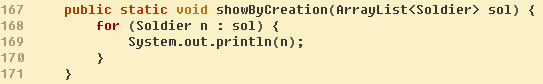
\includegraphics[width=0.99\textwidth,keepaspectratio]{img/showByCreation.png}
		%\includesvg{img/automata.svg}
		%\label{img:mot2}
		%\caption{Product backlog.}
	\end{figure}
	
	\begin{itemize}	
		\item showByCreation(): Básicamente imprime los datos de un ArrayList unidimensional de tipo Soldier.
	\end{itemize}
	
	\begin{figure}[H]
		\centering
		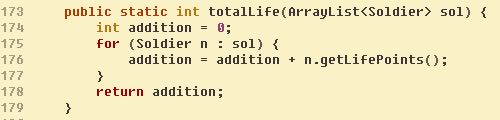
\includegraphics[width=0.99\textwidth,keepaspectratio]{img/totalLife.png}
		%\includesvg{img/automata.svg}
		%\label{img:mot2}
		%\caption{Product backlog.}
	\end{figure}	
	
	
	\begin{itemize}	
		\item totalLife(): El método devuelve los puntos de vida total del ejército. Se decide hacer el método con retorno para poder usar esos valores para determinar al ganador y calcular el promedio.
	\end{itemize}
		
		
		
		
		
	\begin{figure}[H]
		\centering
		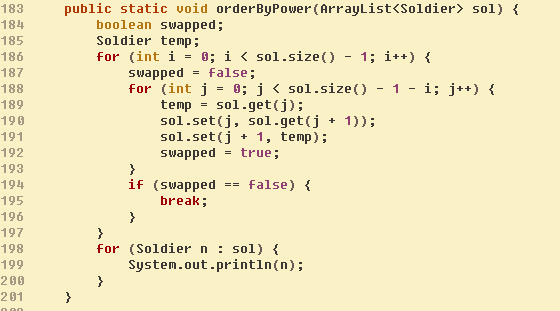
\includegraphics[width=0.98\textwidth,keepaspectratio]{img/orderByPower.png}
		%\includesvg{img/automata.svg}
		%\label{img:mot2}
		%\caption{Product backlog.}
	\end{figure}
	
	\begin{figure}[H]
		\centering
		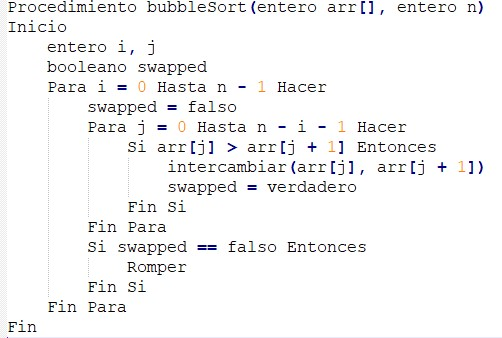
\includegraphics[width=0.9\textwidth,keepaspectratio]{img/burbuja.jpg}
		%\includesvg{img/automata.svg}
		%\label{img:mot2}
		%\caption{Product backlog.}
	\end{figure}
	
	
	\begin{itemize}	
		\item orderByPower(): El método ordena el ArrayList tomando como criterio los puntos de Vida. No se retorna nada
		\item Se muestra el pseudocódigo, pero aplicado a un arreglo Estándar. A pesar de ser otra estructura, la idea es la misma.
	\end{itemize}
		
		

	
	
	\begin{figure}[H]
		\centering
		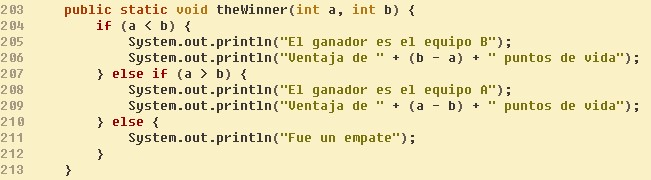
\includegraphics[width=1.1\textwidth,keepaspectratio]{img/theWinner.jpg}
		%\includesvg{img/automata.svg}
		%\label{img:mot2}
		%\caption{Product backlog.}
	\end{figure}
	
	\begin{itemize}	
		\item the Winner(): Este método recibe como parámetros dos enteros los cuales representan los puntos de vida total de cada ejército.Con ayuda de una estructura condicional se imprime un mensaje indicando al ganador o si hubo empate.
	\end{itemize}
	
	

aaaaaaaaaaaaaaaaaa	
	
	
	\subsection{Desarrollo de nuevas funcionalidades}
	
	\begin{lstlisting}[language=bash,caption={Se añaden atributos a la clase Soldier y se crean constructores }][H]
		vim Soldier.java
	\end{lstlisting}
	
	\begin{figure}[H]
		\centering
		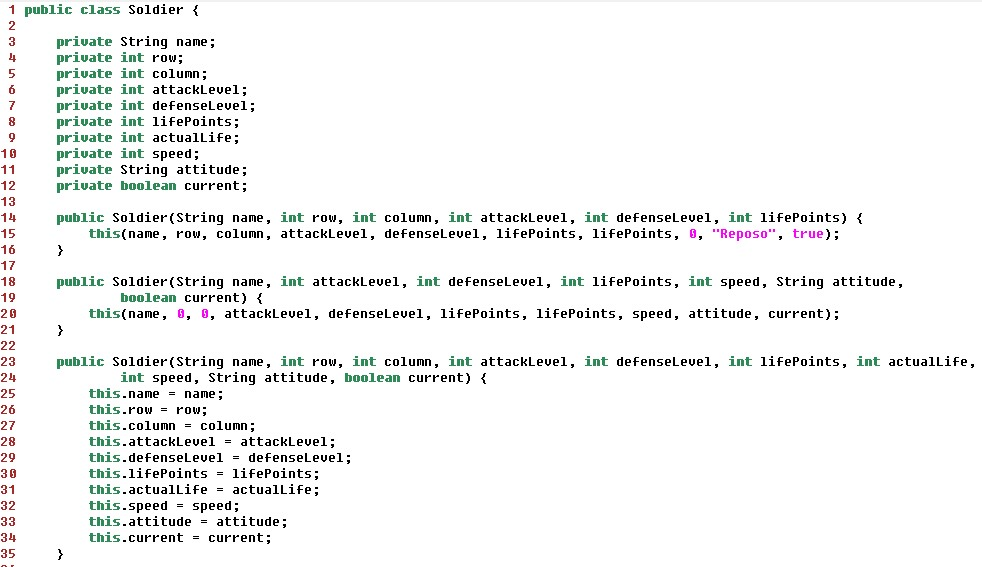
\includegraphics[width=1\textwidth,keepaspectratio]{img/atributos.jpg}
		%\includesvg{img/automata.svg}
		%\label{img:mot2}
		%\caption{Product backlog.}
	\end{figure}
	
	\begin{itemize}	
		\item Por especificaciones del problema se aumentan los atributos attackLevel (nivel de ataque), defenseLevel (nivel de defensa), actuaLife (la vida actual después de un combate por ejemplo), speed (la velocidad), attitude (si está en modo de ataque, huida o defensa), current (si el soldado está vivo).
		\item En cuanto a los constructores. el de la línea 23, se añaden como parámetro todos los atributos. Otro constructor que lo usaremos en el main el cual contiene todo a excepción de actualLife, speed, current, attitude. Por último, se crea un constructor que no se usará mucho, sin embargo, por especificaciones del problema se crea.
	\end{itemize}
	
	\begin{lstlisting}[language=bash,caption={Commit: 73ad0ec83d4c273a3169b0c15ec68c6e4dd9d2a2}][H]
		git add Soldier.java
		git commit -m "Se aumentan atributos nuevos a la clase y tambien los constructores"			
		git push -u origin main
	\end{lstlisting}
	
	
	\begin{lstlisting}[language=bash,caption={Se crea un método que nos muestre los datos de un Soldier }][H]
		vim Soldier.java
	\end{lstlisting}
	
	\begin{figure}[H]
		\centering
		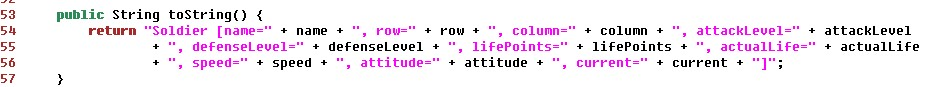
\includegraphics[width=1\textwidth,keepaspectratio]{img/toString.jpg}
		%\includesvg{img/automata.svg}
		%\label{img:mot2}
		%\caption{Product backlog.}
	\end{figure}
	
	\begin{itemize}	
		\item El método toString muestra los datos del soldier.
	\end{itemize}
	
	\begin{lstlisting}[language=bash,caption={Commit: 4ca2b91b8555fdaa32a7abd4c96c4803e64602dd7 }][H]
		git add Soldier.java
		git commit -m "Se aumentan atributos a toString"			
		git push -u origin main
	\end{lstlisting}
	
	
	
	\begin{lstlisting}[language=bash,caption={Se crea el metodo avanzar}][H]
		vim Soldier.java
	\end{lstlisting}
	
	\begin{figure}[H]
		\centering
		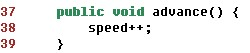
\includegraphics[width=0.5\textwidth,keepaspectratio]{img/advance.jpg}
		%\includesvg{img/automata.svg}
		%\label{img:mot2}
		%\caption{Product backlog.}
	\end{figure}
	
	\begin{itemize}	
		\item Las instrucciones que ofrece la prácticas son muy breves, por lo que se limitó en seguir la instrucción que se nos da para la creación de este método. El método lo que hace es aumentar la velocidad en uno.
	\end{itemize}
	
	\begin{lstlisting}[language=bash,caption={Commit: f024c49ff16d97ebf6611820a92ef6af6587f67c }][H]
		git add Soldier.java
		git commit -m "Se crea el metodo advance"			
		git push -u origin main
	\end{lstlisting}
	
	
	\begin{lstlisting}[language=bash,caption={Se crea el metodo atacar}][H]
		vim Soldier.java
	\end{lstlisting}
	
	\begin{figure}[H]
		\centering
		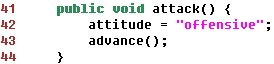
\includegraphics[width=0.5\textwidth,keepaspectratio]{img/attack.jpg}
		%\includesvg{img/automata.svg}
		%\label{img:mot2}
		%\caption{Product backlog.}
	\end{figure}
	
	\begin{itemize}	
		\item Según las instrucciones de la práctica, este método cambiará la actitud del Soldier a modo ofensivo, además de que la velocidad aumentará.
	\end{itemize}
	
	\begin{lstlisting}[language=bash,caption={Commit: cf63faddd8443e7dcdd2cb62635b177373842e61d }][H]
		git add Soldier.java
		git commit -m "Se cambian el nombre de la actitud del metodo attack"			
		git push -u origin main
	\end{lstlisting}
	
	
	
	\begin{lstlisting}[language=bash,caption={Se crea el metodo defender}][H]
		vim Soldier.java
	\end{lstlisting}
	
	\begin{figure}[H]
		\centering
		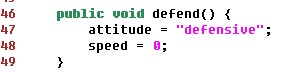
\includegraphics[width=0.5\textwidth,keepaspectratio]{img/defend.jpg}
		%\includesvg{img/automata.svg}
		%\label{img:mot2}
		%\caption{Product backlog.}
	\end{figure}
	
	\begin{itemize}	
		\item Según las instrucciones de la práctica, este método cambiará la actitud del Soldier a modo defensivo, además de que la velocidad será igual a 0.
	\end{itemize}
	
	\begin{lstlisting}[language=bash,caption={Commit: 6b573ae3b1c0241a758325f55f311e19e76361f3 }][H]
		git add Soldier.java
		git commit -m "Se crea el metodo defend"			
		git push -u origin main
	\end{lstlisting}
	
	
		
	\begin{lstlisting}[language=bash,caption={Se crea el metodo retroceder}][H]
		vim Soldier.java
	\end{lstlisting}
	
	\begin{figure}[H]
		\centering
		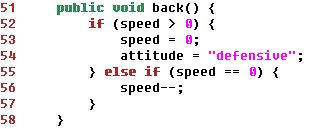
\includegraphics[width=0.5\textwidth,keepaspectratio]{img/back.jpg}
		%\includesvg{img/automata.svg}
		%\label{img:mot2}
		%\caption{Product backlog.}
	\end{figure}
	
	\begin{itemize}	
		\item Según las instrucciones de la práctica, este método cambiará la actitud del Soldier a modo defensivo. Si la velocidad es mayor que 0, el valor se restablece a 0, y si es igual a cero, la velocidad disminuye.
	\end{itemize}
	
	\begin{lstlisting}[language=bash,caption={Commit: f1de159aef9b2d9484f6fcfc3a72032764cc36ab }][H]
		git add Soldier.java
		git commit -m "Metodo back culminado"			
		git push -u origin main
	\end{lstlisting}	
	
			
	\begin{lstlisting}[language=bash,caption={Se crea el metodo morir}][H]
		vim Soldier.java
	\end{lstlisting}
	
	\begin{figure}[H]
		\centering
		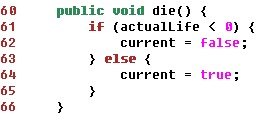
\includegraphics[width=0.5\textwidth,keepaspectratio]{img/die.jpg}
		%\includesvg{img/automata.svg}
		%\label{img:mot2}
		%\caption{Product backlog.}
	\end{figure}
	
	\begin{itemize}	
		\item Según las instrucciones de la práctica, un soldado puede llagar a morir cuando su estado de vida actual tiene un número negativo.
	\end{itemize}
	
	\begin{lstlisting}[language=bash,caption={Commit: 878a442ed1b50d5bf9c8da86d2f096c1128784fd }][H]
		git add Soldier.java
		git commit -m "Se termina el metodo die"			
		git push -u origin main
	\end{lstlisting}	
	
	
	\begin{lstlisting}[language=bash,caption={Se crea el metodo ser atacado}][H]
		vim Soldier.java
	\end{lstlisting}
	
	\begin{figure}[H]
		\centering
		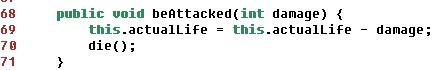
\includegraphics[width=0.8\textwidth,keepaspectratio]{img/beAttacked.jpg}
		%\includesvg{img/automata.svg}
		%\label{img:mot2}
		%\caption{Product backlog.}
	\end{figure}
	
	\begin{itemize}	
		\item Según las instrucciones de la práctica, un soldado cuando es atacado, su vida actual disminuye y puede llegar a morir.
	\end{itemize}
	
	\begin{lstlisting}[language=bash,caption={Commit: 592d758a6eabb49b6bc92d420a6c112081203c4d }][H]
		git add Soldier.java
		git commit -m "Se culmina el metodo beAtacked"			
		git push -u origin main
	\end{lstlisting}
	
	
	\begin{lstlisting}[language=bash,caption={Se crea el metodo huir}][H]
		vim Soldier.java
	\end{lstlisting}
	
	\begin{figure}[H]
		\centering
		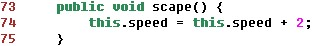
\includegraphics[width=0.8\textwidth,keepaspectratio]{img/scape.jpg}
		%\includesvg{img/automata.svg}
		%\label{img:mot2}
		%\caption{Product backlog.}
	\end{figure}
	
	\begin{itemize}	
		\item Según las instrucciones de la práctica, el método huir hará que la velocidad se incremente en 2.
	\end{itemize}
	
	\begin{lstlisting}[language=bash,caption={Commit: 1da77b3ebe0b75aad7be43592fe92b96918a8ca1 }][H]
		git add Soldier.java
		git commit -m "Se culmina el metodo scape"			
		git push -u origin main
	\end{lstlisting}
	
	
	\begin{lstlisting}[language=bash,caption={Se crean los métodos accesores y mutadores de actualLife}][H]
		vim Soldier.java
	\end{lstlisting}
	
	\begin{figure}[H]
		\centering
		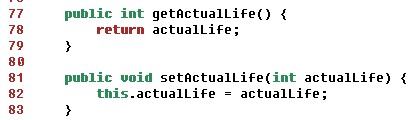
\includegraphics[width=0.8\textwidth,keepaspectratio]{img/actualLife.jpg}
		%\includesvg{img/automata.svg}
		%\label{img:mot2}
		%\caption{Product backlog.}
	\end{figure}
	
	\begin{itemize}	
		\item Según el UML que la práctica propone, estos dos métodos deben estar incluidos.
	\end{itemize}
	
	\begin{lstlisting}[language=bash,caption={Commit: 7ea66af37c1857df332e648e8c1286347fb6cc4b }][H]
		git add Soldier.java
		git commit -m "Se crean los getters y setters de actualLife"			
		git push -u origin main
	\end{lstlisting}
	
	
	
	sssssssssssssssssssssssssssssssssssssssss
	
	\begin{lstlisting}[language=bash,caption={Se corrige el formato de impresión del tablero}][H]
		vim VideoJuego4.java
	\end{lstlisting}
	
	\begin{figure}[H]
		\centering
		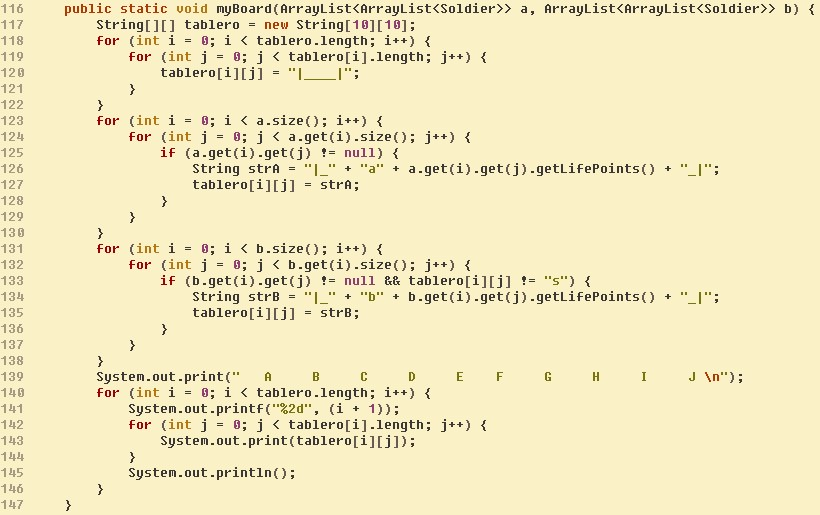
\includegraphics[width=1\textwidth,keepaspectratio]{img/boardComplete.jpg}
		%\includesvg{img/automata.svg}
		%\label{img:mot2}
		%\caption{Product backlog.}
	\end{figure}
	
	\begin{itemize}	
		\item Se aumenta un subguión y la barra vertical tanto en la línea 126 y 134 para que se impriman las casillas donde se ubican los Soldier de forma armónica.
	\end{itemize}
	
	\begin{lstlisting}[language=bash,caption={Compilando y probando el tablero  }][H]
		javac VideoJuego4.java
		java VideoJuego4
		oooooooooooooooo  FASE 1 DE LA CONTIENDA  oooooooooooooooo
		Mostrando estadisticas de cada ejercito
		
		Mostrando soldados por orden de creacion
		DATOS DEL DEL EJERCITO A
		Soldier [name=Soldier1x5, lifePoints=1, row=2, column=6]
		Soldier [name=Soldier3x3, lifePoints=5, row=4, column=4]
		Soldier [name=Soldier5x1, lifePoints=3, row=6, column=2]
		Soldier [name=Soldier6x8, lifePoints=5, row=7, column=9]
		Soldier [name=Soldier7x8, lifePoints=1, row=8, column=9]
		Soldier [name=Soldier9x1, lifePoints=1, row=10, column=2]
		Mayor vida en A: Soldier [name=Soldier6x8, lifePoints=5, row=7, column=9]
		El total de vida del ejercito A es: 16
		El promedio de vida del ejercito A es: 2.6666666666666665
		Mostrando soldados por ranking de poder de A
		Soldier [name=Soldier6x8, lifePoints=5, row=7, column=9]
		Soldier [name=Soldier3x3, lifePoints=5, row=4, column=4]
		Soldier [name=Soldier5x1, lifePoints=3, row=6, column=2]
		Soldier [name=Soldier9x1, lifePoints=1, row=10, column=2]
		Soldier [name=Soldier7x8, lifePoints=1, row=8, column=9]
		Soldier [name=Soldier1x5, lifePoints=1, row=2, column=6]
		
		DATOS DEL EJRCITO B
		Soldier [name=Soldier3x6, lifePoints=1, row=4, column=7]
		Mayor vida en B: Soldier [name=Soldier3x6, lifePoints=1, row=4, column=7]
		El total de vida del ejercito B es: 1
		El promedio de vida del ejercito B es: 1.0
		Mostrando soldados por ranking de poder de B
		Soldier [name=Soldier3x6, lifePoints=1, row=4, column=7]
		
		oooooooooooooooo  FASE 2 DE LA CONTIENDA  oooooooooooooooo
		Mostrando el tablero de juego
		    A     B      C     D      E      F     G      H     I      J
		1 |____||____||____||____||____||____||____||____||____||____|
		2 |____||____||____||____||____||_a1_||____||____||____||____|
		3 |____||____||____||____||____||____||____||____||____||____|
		4 |____||____||____||_a5_||____||____||_b1_||____||____||____|
		5 |____||____||____||____||____||____||____||____||____||____|
		6 |____||_a3_||____||____||____||____||____||____||____||____|
		7 |____||____||____||____||____||____||____||____||_a5_||____|
		8 |____||____||____||____||____||____||____||____||_a1_||____|
		9 |____||____||____||____||____||____||____||____||____||____|
		10|____||_a1_||____||____||____||____||____||____||____||____|
		
		+++++++++++++++++   FASE 3 DE LA CONTIENDA  +++++++++++++++++
		El ganador se determina en base a los puntos de vida total
		Enfrentamiento
		El ganador es el equipo A
		Ventaja de 15 puntos de vida
	\end{lstlisting}
	
	
	\begin{lstlisting}[language=bash,caption={Commit: 8a5f07948da6ece26389a11919f8118d45bcea51}][H]
		git add VideoJuego4.java
		git commit -m "El tablero fue mejorado"			
		git push -u origin main
	\end{lstlisting}
	
	
	
	
	
	
	
	
	\begin{lstlisting}[language=bash,caption={Se crea un método que valida la respuesta del jugador}][H]
		vim VideoJuego4.java
	\end{lstlisting}
	
	\begin{figure}[H]
		\centering
		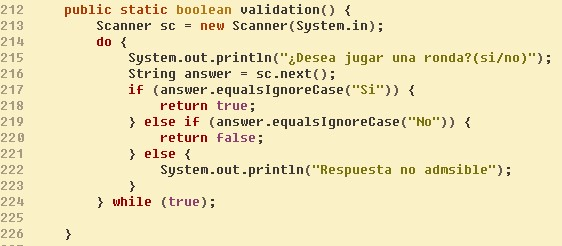
\includegraphics[width=1\textwidth,keepaspectratio]{img/validation.jpg}
		%\includesvg{img/automata.svg}
		%\label{img:mot2}
		%\caption{Product backlog.}
	\end{figure}
	
	\begin{itemize}	
		\item Se crea este método para poder implementar más adelante un ciclo while en el main el cual permitirá que se juegue la cantidad de veces que el usuario deseé. 
		\item En el método se usa el loop do while y una estructura condicional la que retornará un boolean de acuerdo a la respuesta del usuario y para que no hayan errores en las respuestas se usa el método equalsIgnoreCase(Str str) la cual ignora  mayúsculas o minúsculas. Además de que en caso se ingrese una respuesta que no sea "si" o "no" se imprimirá el mensaje de Respuesta no admisible y se repetirá el ciclo hasta que se ingresen los valores correctos.
	\end{itemize}
	
	
	\begin{lstlisting}[language=bash,caption={Commit: 47116e7456c1488e24e11bcd3518f2be3ec47bed}][H]
		git add VideoJuego4.java
		git commit -m "Se mejora el metodo que valida la respuesta del jugador"			
		git push -u origin main
	\end{lstlisting}
	
	
	
	
	
	
	
	\begin{lstlisting}[language=bash,caption={Se implementa el loop While en el main para poder repetir una cantidad n de veces}][H]
		vim VideoJuego4.java
	\end{lstlisting}
	
	\begin{figure}[H]
		\centering
		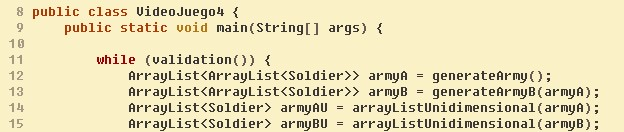
\includegraphics[width=1\textwidth,keepaspectratio]{img/loop.jpg}
		%\includesvg{img/automata.svg}
		%\label{img:mot2}
		%\caption{Product backlog.}
	\end{figure}
	
	\begin{itemize}	
		\item No hay grandes cambios en el main porque solo se mete todo lo que ya estaba en el loop (ver línea 11 de la imagen)
		\item En la condición del while se usa el método validation() para que el loop pueda funcionar de forma correcta sin causar un bucle infinito
	\end{itemize}
	
	\begin{lstlisting}[language=bash,caption={Compilando y probando  }][H]
		javac VideoJuego4.java
		java VideoJuego4
		Desea jugar una ronda?(si/no)
		si
		oooooooooooooooo  FASE 1 DE LA CONTIENDA  oooooooooooooooo
		Mostrando estadisticas de cada ejercito
		
		Mostrando soldados por orden de creacion
		DATOS DEL DEL EJERCITO A
		Soldier [name=Soldier0x4, lifePoints=2, row=1, column=5]
		Soldier [name=Soldier0x8, lifePoints=1, row=1, column=9]
		Soldier [name=Soldier0x9, lifePoints=4, row=1, column=10]
		Soldier [name=Soldier1x7, lifePoints=2, row=2, column=8]
		Soldier [name=Soldier2x1, lifePoints=3, row=3, column=2]
		Soldier [name=Soldier2x7, lifePoints=4, row=3, column=8]
		Soldier [name=Soldier3x9, lifePoints=5, row=4, column=10]
		Soldier [name=Soldier5x8, lifePoints=1, row=6, column=9]
		Soldier [name=Soldier6x3, lifePoints=3, row=7, column=4]
		Soldier [name=Soldier8x9, lifePoints=4, row=9, column=10]
		Mayor vida en A: Soldier [name=Soldier3x9, lifePoints=5, row=4, column=10]
		El total de vida del ejercito A es: 29
		El promedio de vida del ejercito A es: 2.9
		Mostrando soldados por ranking de poder de A
		Soldier [name=Soldier3x9, lifePoints=5, row=4, column=10]
		Soldier [name=Soldier8x9, lifePoints=4, row=9, column=10]
		Soldier [name=Soldier2x7, lifePoints=4, row=3, column=8]
		Soldier [name=Soldier0x9, lifePoints=4, row=1, column=10]
		Soldier [name=Soldier6x3, lifePoints=3, row=7, column=4]
		Soldier [name=Soldier2x1, lifePoints=3, row=3, column=2]
		Soldier [name=Soldier1x7, lifePoints=2, row=2, column=8]
		Soldier [name=Soldier0x4, lifePoints=2, row=1, column=5]
		Soldier [name=Soldier5x8, lifePoints=1, row=6, column=9]
		Soldier [name=Soldier0x8, lifePoints=1, row=1, column=9]
		
		DATOS DEL EJRCITO B
		Soldier [name=Soldier0x5, lifePoints=2, row=1, column=6]
		Soldier [name=Soldier1x3, lifePoints=5, row=2, column=4]
		Soldier [name=Soldier3x8, lifePoints=1, row=4, column=9]
		Mayor vida en B: Soldier [name=Soldier1x3, lifePoints=5, row=2, column=4]
		El total de vida del ejercito B es: 8
		El promedio de vida del ejercito B es: 2.6666666666666665
		Mostrando soldados por ranking de poder de B
		Soldier [name=Soldier1x3, lifePoints=5, row=2, column=4]
		Soldier [name=Soldier0x5, lifePoints=2, row=1, column=6]
		Soldier [name=Soldier3x8, lifePoints=1, row=4, column=9]
		
		oooooooooooooooo  FASE 2 DE LA CONTIENDA  oooooooooooooooo
		Mostrando el tablero de juego
		   A      B      C     D      E      F     G      H     I      J
		1 |____||____||____||____||_a2_||_b2_||____||____||_a1_||_a4_|
		2 |____||____||____||_b5_||____||____||____||_a2_||____||____|
		3 |____||_a3_||____||____||____||____||____||_a4_||____||____|
		4 |____||____||____||____||____||____||____||____||_b1_||_a5_|
		5 |____||____||____||____||____||____||____||____||____||____|
		6 |____||____||____||____||____||____||____||____||_a1_||____|
		7 |____||____||____||_a3_||____||____||____||____||____||____|
		8 |____||____||____||____||____||____||____||____||____||____|
		9 |____||____||____||____||____||____||____||____||____||_a4_|
		10|____||____||____||____||____||____||____||____||____||____|
		
		+++++++++++++++++   FASE 3 DE LA CONTIENDA  +++++++++++++++++
		El ganador se determina en base a los puntos de vida total
		Enfrentamiento
		El ganador es el equipo A
		Ventaja de 21 puntos de vida
		Desea jugar una ronda?(si/no)
		7 
		Respuesta no admsible
		Desea jugar una ronda?(si/no)
		no
	\end{lstlisting}
 

	\begin{lstlisting}[language=bash,caption={Commit: 41ffd9ca2d4934c86227d650940d5a93865bc037}][H]
		git add VideoJuego3.java
		git commit -m "Se crea el loop que permite jugar n cantidad de veces"			
		git push -u origin main
	\end{lstlisting}

	
	
	
	
	
	
		
	\begin{lstlisting}[language=bash,caption={Se implementa un método que realiza una búsqueda Binaria según el nombre}][H]
		vim VideoJuego4.java
	\end{lstlisting}
	
	\lstinputlisting[language=Java,numbers=left,]{src/binary.java}
	
	
	\begin{itemize}	
		\item Este es el pseudocódigo general de la búsqueda binaria.
	\end{itemize}
	
	
	
	\begin{figure}[H]
		\centering
		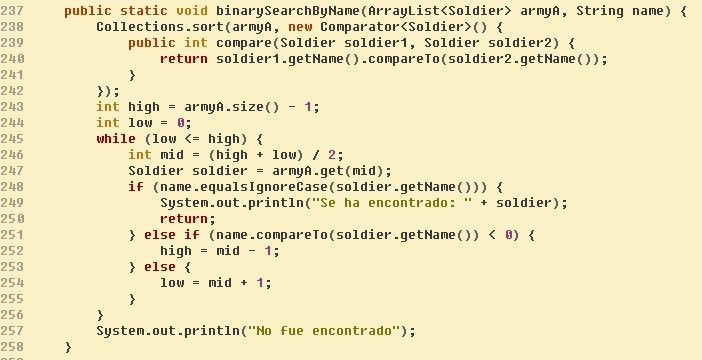
\includegraphics[width=1\textwidth,keepaspectratio]{img/binarySearch.jpg}
		%\includesvg{img/automata.svg}
		%\label{img:mot2}
		%\caption{Product backlog.}
	\end{figure}
	
	\begin{itemize}	
		\item Para una mejor presentación del código, se decide por solo limitarse a mostrar mensajes al usuario y colocar los métodos en el main, esa es la razón por la que se decide hacer este método sin retorno.
		\item  Pese a contar con un método de ordenamiento, ese es de tipo void, así que  para ordenar este arreglo y hacer la búsqueda binaria, se tendrá que hacerlo en el mismo método, por lo que se hará uso del método Collections.sort del cual se hará una personalización en el parámetro de Comparator haciendo que el criterio sean los nombres de cada Soldier.
	\end{itemize}
	
	\begin{lstlisting}[language=bash,caption={Compilando y probando  }][H]
		javac VideoJuego4.java
		java VideoJuego4
		Desea jugar una ronda?(si/no)
		si
		oooooooooooooooo  FASE 1 DE LA CONTIENDA  oooooooooooooooo
		Mostrando estadisticas de cada ejercito
		
		Mostrando soldados por orden de creacion
		DATOS DEL DEL EJERCITO A
		Soldier [name=Soldier0x1, lifePoints=3, row=1, column=2]
		Soldier [name=Soldier1x4, lifePoints=4, row=2, column=5]
		Soldier [name=Soldier2x9, lifePoints=1, row=3, column=10]
		Soldier [name=Soldier5x6, lifePoints=3, row=6, column=7]
		Soldier [name=Soldier7x4, lifePoints=5, row=8, column=5]
		Soldier [name=Soldier9x0, lifePoints=5, row=10, column=1]
		Soldier [name=Soldier9x4, lifePoints=5, row=10, column=5]
		Mayor vida en A: Soldier [name=Soldier9x4, lifePoints=5, row=10, column=5]
		El total de vida del ejercito A es: 26
		El promedio de vida del ejercito A es: 3.7142857142857144
		Mostrando soldados por ranking de poder de A
		Soldier [name=Soldier9x4, lifePoints=5, row=10, column=5]
		Soldier [name=Soldier9x0, lifePoints=5, row=10, column=1]
		Soldier [name=Soldier7x4, lifePoints=5, row=8, column=5]
		Soldier [name=Soldier1x4, lifePoints=4, row=2, column=5]
		Soldier [name=Soldier5x6, lifePoints=3, row=6, column=7]
		Soldier [name=Soldier0x1, lifePoints=3, row=1, column=2]
		Soldier [name=Soldier2x9, lifePoints=1, row=3, column=10]
		Ingrese el nombre del Soldier que desea buscar
		Soldier0x1
		Se ha encontrado: Soldier [name=Soldier0x1, lifePoints=3, row=1, column=2]
		
		DATOS DEL EJRCITO B
		Soldier [name=Soldier6x3, lifePoints=5, row=7, column=4]
		Mayor vida en B: Soldier [name=Soldier6x3, lifePoints=5, row=7, column=4]
		El total de vida del ejercito B es: 5
		El promedio de vida del ejercito B es: 5.0
		Mostrando soldados por ranking de poder de B
		Soldier [name=Soldier6x3, lifePoints=5, row=7, column=4]
		Ingrese el nombre del Soldier que desea buscar
		oooooooooooooooo  FASE 2 DE LA CONTIENDA  oooooooooooooooo
		Mostrando el tablero de juego
		   A      B      C     D      E      F     G      H     I      J
		1 |____||_a3_||____||____||____||____||____||____||____||____|
		2 |____||____||____||____||_a4_||____||____||____||____||____|
		3 |____||____||____||____||____||____||____||____||____||_a1_|
		4 |____||____||____||____||____||____||____||____||____||____|
		5 |____||____||____||____||____||____||____||____||____||____|
		6 |____||____||____||____||____||____||_a3_||____||____||____|
		7 |____||____||____||_b5_||____||____||____||____||____||____|
		8 |____||____||____||____||_a5_||____||____||____||____||____|
		9 |____||____||____||____||____||____||____||____||____||____|
		10|_a5_||____||____||____||_a5_||____||____||____||____||____|
		
		+++++++++++++++++   FASE 3 DE LA CONTIENDA  +++++++++++++++++
		El ganador se determina en base a los puntos de vida total
		Enfrentamiento
		El ganador es el equipo A
		Ventaja de 21 puntos de vida
		Desea jugar una ronda?(si/no)
		NO
	\end{lstlisting}
	
	
	\begin{lstlisting}[language=bash,caption={Commit: dde0af374ba825d7f45cb32605658c8624920f51}][H]
		git add VideoJuego4.java
		git commit -m "Se culmina el metodo binarySearcByName"			
		git push -u origin main
	\end{lstlisting}
	
	
	
	
			
	\begin{lstlisting}[language=bash,caption={Se implementa un método que realiza una búsqueda secuencial según el nombre}][H]
		vim VideoJuego4.java
	\end{lstlisting}
	
	
	\begin{figure}[H]
		\centering
		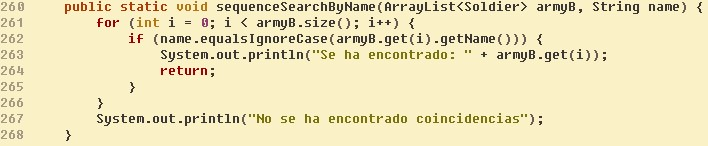
\includegraphics[width=1\textwidth,keepaspectratio]{img/sequence.jpg}
		%\includesvg{img/automata.svg}
		%\label{img:mot2}
		%\caption{Product backlog.}
	\end{figure}
	
	\begin{itemize}	
		\item Este método busca a lo largo del ArrayList elemento por elemento. La búsqueda secuencial no es una buena opción debido a que hace recorridos demás. Se lo emplea más que nada porque los objetivos de la práctica lo exigen.
	\end{itemize}
	
	\begin{lstlisting}[language=bash,caption={Compilando y probando el código terminado  }][H]
		javac VideoJuego4.java
		java VideoJuego4
		Desea jugar una ronda?(si/no)
		SI
		oooooooooooooooo  FASE 1 DE LA CONTIENDA  oooooooooooooooo
		Mostrando estadisticas de cada ejercito
		
		Mostrando soldados por orden de creacion
		DATOS DEL DEL EJERCITO A
		Soldier [name=Soldier5x2, lifePoints=2, row=6, column=3]
		Soldier [name=Soldier9x8, lifePoints=1, row=10, column=9]
		Mayor vida en A: Soldier [name=Soldier5x2, lifePoints=2, row=6, column=3]
		El total de vida del ejercito A es: 3
		El promedio de vida del ejercito A es: 1.5
		Mostrando soldados por ranking de poder de A
		Soldier [name=Soldier5x2, lifePoints=2, row=6, column=3]
		Soldier [name=Soldier9x8, lifePoints=1, row=10, column=9]
		Ingrese el nombre del Soldier que desea buscar
		soldier5x2
		Se ha encontrado: Soldier [name=Soldier5x2, lifePoints=2, row=6, column=3]
		
		DATOS DEL EJRCITO B
		Soldier [name=Soldier2x9, lifePoints=5, row=3, column=10]
		Soldier [name=Soldier3x1, lifePoints=3, row=4, column=2]
		Soldier [name=Soldier3x5, lifePoints=2, row=4, column=6]
		Soldier [name=Soldier3x7, lifePoints=3, row=4, column=8]
		Soldier [name=Soldier4x2, lifePoints=1, row=5, column=3]
		Soldier [name=Soldier5x0, lifePoints=1, row=6, column=1]
		Soldier [name=Soldier5x8, lifePoints=1, row=6, column=9]
		Soldier [name=Soldier7x4, lifePoints=1, row=8, column=5]
		Mayor vida en B: Soldier [name=Soldier2x9, lifePoints=5, row=3, column=10]
		El total de vida del ejercito B es: 17
		El promedio de vida del ejercito B es: 2.125
		Mostrando soldados por ranking de poder de B
		Soldier [name=Soldier2x9, lifePoints=5, row=3, column=10]
		Soldier [name=Soldier3x7, lifePoints=3, row=4, column=8]
		Soldier [name=Soldier3x1, lifePoints=3, row=4, column=2]
		Soldier [name=Soldier3x5, lifePoints=2, row=4, column=6]
		Soldier [name=Soldier7x4, lifePoints=1, row=8, column=5]
		Soldier [name=Soldier5x8, lifePoints=1, row=6, column=9]
		Soldier [name=Soldier5x0, lifePoints=1, row=6, column=1]
		Soldier [name=Soldier4x2, lifePoints=1, row=5, column=3]
		Ingrese el nombre del Soldier que desea buscar
		soldier4x2
		Se ha encontrado: Soldier [name=Soldier4x2, lifePoints=1, row=5, column=3]
		
		oooooooooooooooo  FASE 2 DE LA CONTIENDA  oooooooooooooooo
		Mostrando el tablero de juego
	       A      B      C     D      E      F     G      H     I      J
		1 |____||____||____||____||____||____||____||____||____||____|
		2 |____||____||____||____||____||____||____||____||____||____|
		3 |____||____||____||____||____||____||____||____||____||_b5_|
		4 |____||_b3_||____||____||____||_b2_||____||_b3_||____||____|
		5 |____||____||_b1_||____||____||____||____||____||____||____|
		6 |_b1_||____||_a2_||____||____||____||____||____||_b1_||____|
		7 |____||____||____||____||____||____||____||____||____||____|
		8 |____||____||____||____||_b1_||____||____||____||____||____|
		9 |____||____||____||____||____||____||____||____||____||____|
		10|____||____||____||____||____||____||____||____||_a1_||____|
		
		+++++++++++++++++   FASE 3 DE LA CONTIENDA  +++++++++++++++++
		El ganador se determina en base a los puntos de vida total
		Enfrentamiento
		El ganador es el equipo B
		Ventaja de 14 puntos de vida
		Desea jugar una ronda?(si/no)
		no
	\end{lstlisting}
	
	\begin{lstlisting}[language=bash,caption={Commit: 5575a0d5eead5b5dd4dca7425a5b9f37229e25fa}][H]
		git add VideoJuego4.java
		git commit -m "Se culima el metood sequenceSearchByName"			
		git push -u origin main
	\end{lstlisting}
	
	
	\subsection{Diagrama UML y el main}
	
	\begin{figure}[H]
		\centering
		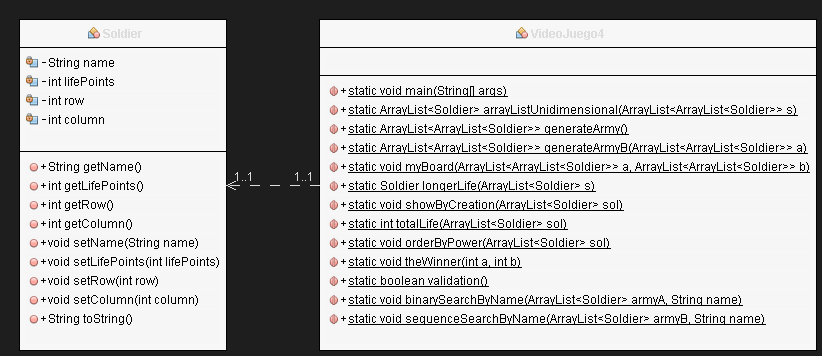
\includegraphics[width=1\textwidth,keepaspectratio]{img/uml.png}
		%\includesvg{img/automata.svg}
		%\label{img:mot2}
		%\caption{Product backlog.}
	\end{figure}
	

		\begin{figure}[H]
		\centering
		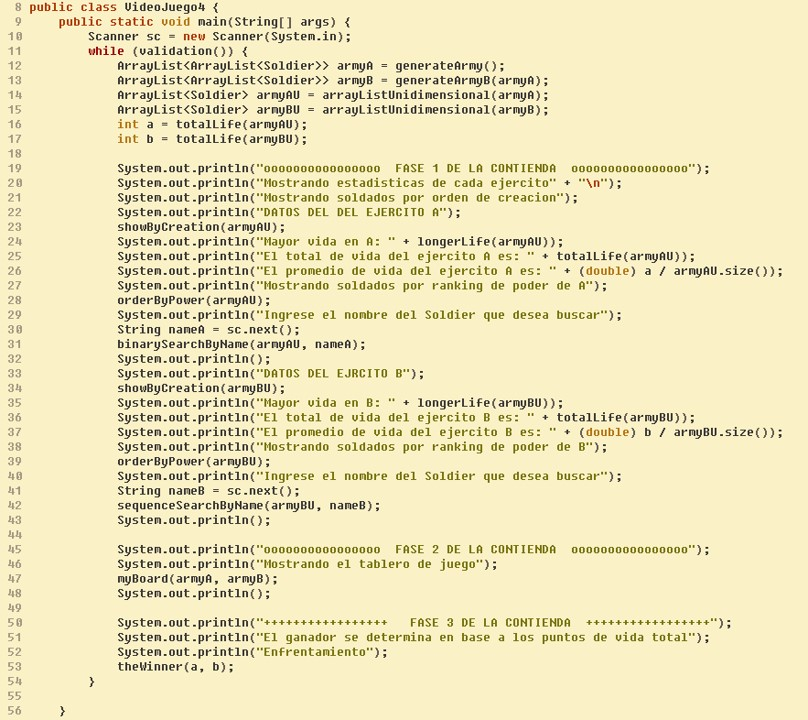
\includegraphics[width=1\textwidth,keepaspectratio]{img/main.jpg}
		%\includesvg{img/automata.svg}
		%\label{img:mot2}
		%\caption{Product backlog.}
	\end{figure}
	


	
	\subsection{Estructura de laboratorio 07}
	\begin{itemize}	
		\item El contenido que se entrega en este laboratorio es el siguiente:
	\end{itemize}
	
	\begin{lstlisting}[style=ascii-tree]
		lab08
		|    Soldier.java
		|
		|    VideoJuego4.java
		|
		 ──latex
				|   	programacion_lab07_rescobedoq_v1.0.pdf
				|   	programacion_lab07_rescobedoq_v1.0.tex
				|
				|----img
				|         arrayListUni.jpg
				|         binarySearch.jpg
				|         board.jpg
				|         boardComplete.jpg
				|         burbuja.jpg
				|         generateArmy.jpg
				|         generateArmyB.jpg
				|         insertion.jpg
				|         logo_abet.png
				|         logo_episunsa.png
				|         logo_unsa.jpg
				|         longerLife.png
				|         loop.jpg
				|         main.jpg
				|         orderByPower.png
				|         sequence.jpg
				|         showByCreation.png
				|         theWinner.jpg
				|         totalLife.png
				|         uml.png
				|         validation.jpg
				|
				 ───src
							 binary.java	
			
		
	\end{lstlisting}    
	
	\section{\textcolor{red}{Rúbricas}}
	
	\subsection{\textcolor{red}{Entregable Informe}}
	\begin{table}[H]
		\caption{Tipo de Informe}
		\setlength{\tabcolsep}{0.5em} % for the horizontal padding
		{\renewcommand{\arraystretch}{1.5}% for the vertical padding
			\begin{tabular}{|p{3cm}|p{12cm}|}
				\hline
				\multicolumn{2}{|c|}{\textbf{\textcolor{red}{Informe}}}  \\
				\hline 
				\textbf{\textcolor{red}{Latex}} & \textcolor{blue}{El informe está en formato PDF desde Latex,  con un formato limpio (buena presentación) y facil de leer.}   \\ 
				\hline 
				
				
			\end{tabular}
		}
	\end{table}
	
	\clearpage
	
	\subsection{\textcolor{red}{Rúbrica para el contenido del Informe y demostración}}
	\begin{itemize}			
		\item El alumno debe marcar o dejar en blanco en celdas de la columna \textbf{Checklist} si cumplio con el ítem correspondiente.
		\item Si un alumno supera la fecha de entrega,  su calificación será sobre la nota mínima aprobada, siempre y cuando cumpla con todos lo items.
		\item El alumno debe autocalificarse en la columna \textbf{Estudiante} de acuerdo a la siguiente tabla:
		
		\begin{table}[ht]
			\caption{Niveles de desempeño}
			\begin{center}
				\begin{tabular}{ccccc}
					\hline
					& \multicolumn{4}{c}{Nivel}\\
					\cline{1-5}
					\textbf{Puntos} & Insatisfactorio 25\%& En Proceso 50\% & Satisfactorio 75\% & Sobresaliente 100\%\\
					\textbf{2.0}&0.5&1.0&1.5&2.0\\
					\textbf{4.0}&1.0&2.0&3.0&4.0\\
					\hline
				\end{tabular}
			\end{center}
		\end{table}	
		
	\end{itemize}
	
	\begin{table}[H]
		\caption{Rúbrica para contenido del Informe y demostración}
		\setlength{\tabcolsep}{0.5em} % for the horizontal padding
		{\renewcommand{\arraystretch}{1.5}% for the vertical padding
			%\begin{center}
			\begin{tabular}{|p{2.7cm}|p{7cm}|x{1.3cm}|p{1.2cm}|p{1.5cm}|p{1.1cm}|}
				\hline
				\multicolumn{2}{|c|}{Contenido y demostración} & Puntos & Checklist & Estudiante & Profesor\\
				\hline
				\textbf{1. GitHub} & Hay enlace URL activo del directorio para el  laboratorio hacia su repositorio GitHub con código fuente terminado y fácil de revisar. &2 &X &2 & \\ 
				\hline
				\textbf{2. Commits} &  Hay capturas de pantalla de los commits más importantes con sus explicaciones detalladas. (El profesor puede preguntar para refrendar calificación). &4 &X &4 & \\ 
				\hline 
				\textbf{3. Código fuente} &  Hay porciones de código fuente importantes con numeración y explicaciones detalladas de sus funciones. &2 &X &2 & \\ 
				\hline 
				\textbf{4. Ejecución} & Se incluyen ejecuciones/pruebas del código fuente  explicadas gradualmente. &2 &X &2 & \\ 
				\hline			
				\textbf{5. Pregunta} & Se responde con completitud a la pregunta formulada en la tarea.  (El profesor puede preguntar para refrendar calificación).  &2 &X &2 & \\ 
				\hline	
				\textbf{6. Fechas} & Las fechas de modificación del código fuente estan dentro de los plazos de fecha de entrega establecidos. &2 &X &2 & \\ 
				\hline 
				\textbf{7. Ortografía} & El documento no muestra errores ortográficos. &2 &X &1 & \\ 
				\hline 
				\textbf{8. Madurez} & El Informe muestra de manera general una evolución de la madurez del código fuente,  explicaciones puntuales pero precisas y un acabado impecable.   (El profesor puede preguntar para refrendar calificación).  &4 &X &3 & \\ 
				\hline
				\multicolumn{2}{|c|}{\textbf{Total}} &20 & &18 & \\ 
				\hline
			\end{tabular}
			%\end{center}
			%\label{tab:multicol}
		}
	\end{table}
	
	\clearpage
	
	\section{Referencias}
	\begin{itemize}			
		\item \url{https://www.geeksforgeeks.org/bubble-sort/}
		\item \url{https://www.geeksforgeeks.org/insertion-sort/}
	\end{itemize}	
	
	%\clearpage
	%\bibliographystyle{apalike}
	%\bibliographystyle{IEEEtranN}
	%\bibliography{bibliography}
	
\end{document}